% -*- root: ../../main.tex -*-
\section{File Manager}
\label{sec:file_manager_design}
A seguito di un analisi dei file utilizzati e delle varie risorse caricate da jar e non, sono state individuate tre principali \textbf{categorie} di operazioni.

\hfill \break
Operazioni su:
\begin{enumerate}
    \item \textbf{File generici}
    \item \textbf{File Yaml}
    \item \textbf{Altri dati (musica, sprite, ecc)}
\end{enumerate}

Ogni categoria è gestita con una classe separata: i file generici sono stati gestiti dal \textbf{FileManager}, i file Yaml con lo \textbf{YamlManager} e gli altri dati con il \textbf{DataManager}.


\begin{figure}[H]
	\centering
	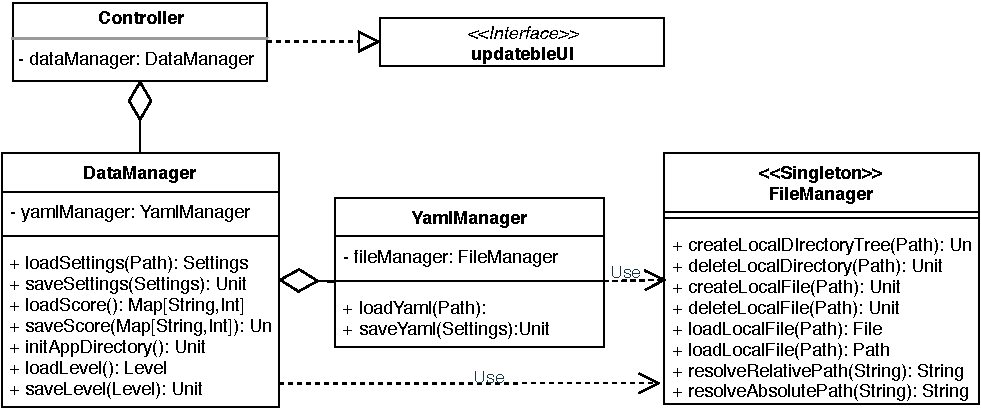
\includegraphics[width=0.90\columnwidth]{drawio/fileManager/fileManager.pdf}
	\caption{Diagramma di classe rappresentante la struttura dei tre manager.}
	\label{fig:FileManager}
\end{figure}

\begin{itemize}
    \item \textbf{FileManager}: le operazioni di \textbf{base} sui file come il \textbf{caricamento} di una risorsa da jar o da sistema, possono essere effettuate da qualunque modulo dell'applicazione.
    
    Un solo FileManager è sufficiente per la gestione dei file in tutto l' applicativo; di conseguenza è stato progettato avvalendosi dell'utilizzo del pattern \textbf{Singleton}.
    Inoltre la divisione dei compiti e l'accesso globale consentono di diminuire il rischio di creare \textbf{God class}.
    \item \textbf{YamlManager}: i file \textbf{Yaml} sono la principale tecnica di \textbf{serializzazione} dei dati utilizzata nel contesto di questo progetto; in essi vengono salvati \textbf{livelli}, \textbf{record} e \textbf{dati utente}.
    Per questo è stato introdotto un \textbf{gestore} unicamente dedicato ai file Yaml che si appoggia sul \texttt{FileManager} per le \textbf{operazioni di base} e ne consente \textbf{scrittura} e \textbf{lettura}.
    \item \textbf{DataManager}: consente l'accesso a tutti i dati \textbf{astratti} del programma (livelli, impostazioni, statistiche, ecc).
    Si basa sullo \texttt{YamlManager} e il \texttt{FileManager} per effettuare le operazioni di caricamento e salvataggio ed è utilizzato dal \textbf{Controller} che lo sfrutta per accedere alle varie risorse \textbf{testuali}.
\end{itemize}